%\addcontentsline{toc}{chapter}{Development Process}
\chapter{Design}
On completion of my analysis and background planning for the project, I can now look at more detailed design for the application overview, and the individual component it comprises of. Because my application will present both a front-end GUI and back-end JavaScript and WebGl, I will split my design into two sections. The reasoning for this is because I would prefer to have the GUI and logic of the application to be decoupled, so that the code can be changed in the JavaScript easily without having to affect the user interface. Other than planning the application itself, it is also important I plan what key assisting services I use, such as how I intend on versioning my code, to how I will deploy my code.

\section{Overall Architecture}
As a summary of the architecture of my planned application, the best way to design in more detail is to lay out a primary design pattern. For the purpose of an application which will allow for user interaction, which will be processed by code in the back-end, I have decided to go ahead with a Model-view-controller approach. Using the MVC pattern means I can separate the GUI from the logic code as I wanted to, and have the GUI exists without knowledge of the back-end. This is also the same with the model, where the primary code for calculating manoeuvre movements and animations should be possible without knowledge of the view, but instead use the controller as a intermediary. See figure ~\ref{fig:mvc} for the MVC pattern I plan to use. 

\begin{figure}[h!]
  \centering
      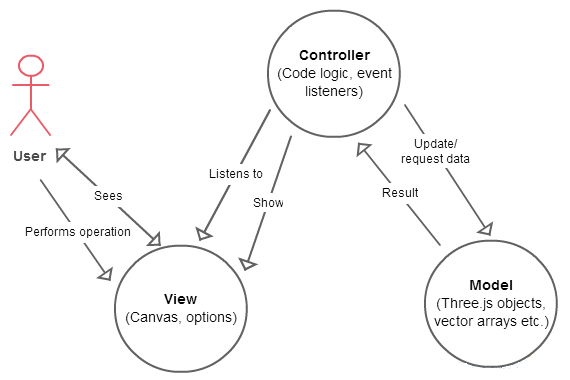
\includegraphics[width=0.8\textwidth]{images/mvc.png}
  \caption{Model View Controller diagram for my proposed application. Shows the planned interactions between different subjects within my application.}
  \label{fig:mvc}
\end{figure}

Because I have already chosen three.js as library of choice for creating any graphics and physics objects, these will already form my model or models. Each manoeuvre for instance will be reflected as a set of vectors which will form the shapes of the Aresti flight paths, and should be accessible and changeable through the controller to the view (in this case the canvas in my GUI).

The controller will be the most crucial part I implement, as it will need to be able to communicate with the three.js objects, the canvas displaying the animation, and detect controls from the user. For this piece of the pattern, I will enforce some other design patterns to 

Finally, the view will be represented as the canvas and controls on the web page. Since on both the canvas and the options menu can have an effect on the model, the controller will listen for changes on either, and then call the relevant operations to affect the model, and again reflect this back onto the view. The view will not know anything of the controller nor the model, so adding any new options or displayable information will be easier and not conflict with any current elements.

\section{Back-end logic and design}
The first of the two design categories concentrates on the JavaScript that will act as the functions to run each of the proposed features of the application. The code on this side will be responsible for maintaining contact with the GUI, and more importantly the WebGL canvas on the web page. To make the code be as maintainable and run effectively as possible, I will look into a variety of design patterns.

\subsection{Design patterns}
Because I am using a hybrid of waterfall and FDD at this stage of the project, using a changing range of design patterns for my JavaScript and GUI architecture is possible. Through the implementation stage of this report, some of these may patterns mentioned may not be used anymore and replaced for different ones depending on changing requirements and progress. Using the implement, refactor and test iteration approach should allow for this.

The first design pattern that would be good useful relating to the controller is known as an observer pattern. The observer pattern means to listen on an event or events in an application, and then call the relevant action. The JQuery library, which I plan to use throughout any GUI related tasks will be of a great use here. This library will allow me to add simple listeners on elements on the web page, and set methods to be called on any click, hover or other events. In terms of how I will place this pattern in my architecture, a standalone file will be responsible for listening to any options or menu changes, whilst another JavaScript file will be responsible for listening to the canvas events such as rotation or zoom. One web article here \cite{observer} supports the advantage that the observer pattern will help towards decoupling.

The next design pattern I plan on implementing into my application relates again to the MVC architecture I will be using. The builder pattern will allow me to append and edit any HTML on the page (such as options, check-boxes, loading content back into the OLAN input box) easily with data retrieved from the model. JQuery again should help to provide a means of changing content, because of more built-in method it comes with. There should be a handler class in my application specifically for controlling the page content.

A third design pattern which will be important when it comes to loading up the application will ensure that all the data necessary to run the application is ready before the user can perform any actions. Known as the Lazy initialisation pattern, this is a style of coding that means whenever files or data is being loaded, the rest of the application should either wait, or prevent other relying features from being initialized. One motivation for the need for this pattern in my program is because of the vast amount of manoeuvre data, and model data for terrain or for aircrafts means that functionality such as animating and drawing flight paths on the canvas may be already ready for use from the user before all the data is ready. In this case, it could cause errors and even crash the application. Therefore, making sure that the application does not progress loading before data is ready is of great importance. Martin fowler mentions this pattern in his site \cite{lazy_initialisation} and whilst says this pattern should be avoided if possible due to responsiveness being hindered, he agrees that this could be used to solve performance problems.

Although the previous design patterns have been chosen, others were considered when planning the application but were not suitable or better options were available. One such pattern, the Mixin pattern allows JavaScript functions to be inherited from other classes or inner functions. For instance, these would be useful as a means of decreasing repetition of functions. In my proposed application, I thought about the possibility of using a Mixin style architecture to allow functions that would draw both the manoeuvres on the canvas, and the manoeuvres on the movie-reel. The reason I have decided not to use this pattern falls to the issue that by making an object extend and hold code from elsewhere could make it harder to maintain, see where the function comes from, and uncertainty of location of any bugs I may come across while developing. While researching other possible design patterns, a book written by Addy Osmani \cite{design_patterns} was especially useful as most known JavaScript design patterns were explained, and their advantages and disadvantages pointed out.

\subsection{Module diagram}
\label{sec:module}
Because much of the code I will be implementing will hold various Three.Js objects, I have decided that modulating methods and objects will be better than simulating classes seeing as JavaScript is a class-less language. This is a pattern known as the module pattern. Although this may appear less object orientated, modules allow for more robust architecture where units of code can be separated and organised. Modules are slightly similar to classes in the way they can hide code that should not be accessible to other modules by encapsulates privacy. When code is modulated, and then that module is called upon by another, only a public API is returned, and other methods in that module are kept private from being used in other parts of the application. These private methods are good for use as supporting methods, holding such things as calculations, or private variables for getters and setters. Again, this is a similar case to the traditional class diagram.

There are currently a selection of libraries that allow for modules in JavaScript. The most prominent, and the one I would like to use is called RequireJS, which promises the increase in speed and quality of code. RequireJS works by dynamically loading JavaScript files on the fly, where the code has from the other module is usable once loaded into the module calling it. Once modules are loaded into an object form in whatever the developer needs to name it, its public variables and methods can then be accessed. See figure ~\ref{fig:module} on how modules are used. In my case, modules would be useful in enforcing the MVC pattern in the way that it will help towards hiding code between the view and the model. 

\lstset{language=JavaScript}
\medskip
\begin{lstlisting}[caption=Example showing how RequireJS loads in another module or JavaScript file which in this case is loading up the util JavaScript module and naming it as object 'util' for use in the code]
require(["helper/util"], function(util) { 
  
  // This function can not be called by another module
  function private_function(){
    util.Method() // Can call public methods in the util file
  }
  return {
    public_function: function(){
      // can be called if this module is loaded into another
    }
  }
});
\end{lstlisting}
\label{fig:module}

In order to create a basis for modulating code, I should first look to separate the features I listed in the analysis section of this report into categories. These categories will then help me to determine how I could structure my application in as best object orientated way as possible.

The categories I have been able to come to are:
\begin{itemize}
  \item Main- initiating other modules, beginning the application.
  \item Animation- Playing, and controlling speed, physics of animation.
  \item Loading manoeuvres at start of application.
  \item Saving and loading animations
  \item Cameras- Creating and controlling cameras movements
  \item GUI controlling- control and edit GUI controls, and appearance from back-end. Also including the possible movie reel live animation.
  \item Canvas controls- Allowing the user to move along the canvas, and zoom.
\end{itemize}

Now I have a stable list of categorised features, I am able to create a diagram shown in figure ~\ref{fig:mod} to represent what modulated layout my application will use. Because of the way modules handle public and private variables, have public and have private methods, means that this is very reminiscent of a standard class diagram.

\clearpage

\begin{figure}[h]
  \centering
      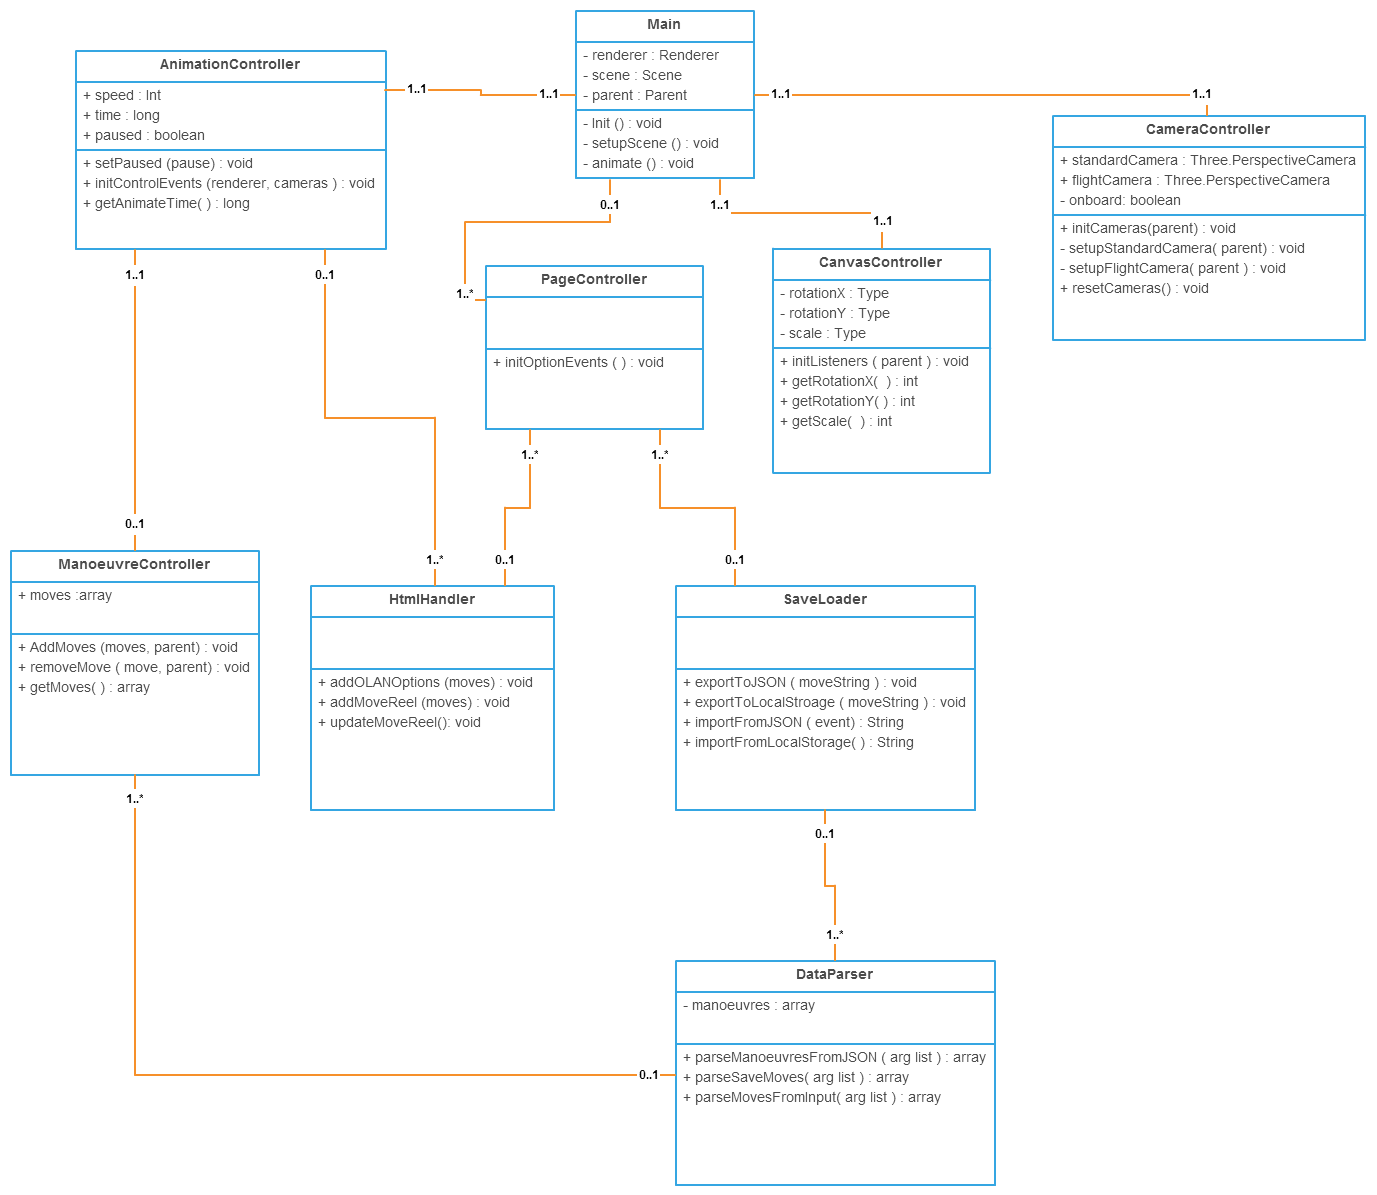
\includegraphics[width=1\textwidth]{images/mod.png}
  \caption{Module diagram displaying the various communications between modules, and how they are connected to the GUI in the MVC way.}
  \label{fig:mod}
\end{figure}

This module diagram shows what will be the communications between modules in the application, providing insight into what each module should contain in terms of important variables and methods. Ensuring that only modules that require certain pieces of information from another module has sole access is important to reinforce the module pattern mentioned earlier. It should be noted here that although the diagram shows the main modules that will oversee most of the features of the application, when implementation occurs later on in the project, more modules or JavaScript files may be added to support or lighten the load of functions. This is supported by the good practice of \textbf{keeping files and functions short and concise} for easier maintenance and readability. The following descriptions have been kept brief, and key connections within the diagram discussed.

The first module proposed from the diagram will be the module entitled 'Main', which will be responsible for setting up the application, and hold onto key variables such as the renderer and scene objects to allow for anything to be drawn and animated on the canvas. This module will be called from the HTML and then will begin any necessary calls to set up the listeners for the cameras, canvas and options. The most important call will be the call to set up the animation controller module. 

Following on, the animation controller module will be one of the largest and most important parts of the overall architecture, as it will be responsible for both animating flight paths, loading up the OLAN manoeuvres at start of the application, and relating any actions from the user to do with OLAN selections or playing and pausing, as well as changing animation speeds. 

The animation controller module will be in communication with the manoeuvre controller, which will be a logic heavy class because of the calculations it will require to compute and construct the sets of vectors of the Aresti shapes representing each OLAN notation. As the diagram shows, the application will first get the user OLAN input from the web page via the HTML handler module, then search via the dataParse module and create the manoeuvres array object within the manoeuvre controller holding all the calculated manoeuvres, and return this in a 'get' method to the animation module for placing on the canvas.

As mentioned earlier, the HTML handler module will be the first means of contact to the user of the application, retrieving input from the OLAN box, getting values of any check-boxes, and also setting any values. This module will be using the JQuery library as well as the Handlebars library as the primary way to communicate with the front-end, by directly referencing ID's of divs on the web page.

Two other controllers that should be mentioned are the camera and canvas modules. Both modules will be responsible for setting up their elements when the application starts up (including the different sets of cameras, locations, lighting and ground effects) and for listening to evens on both of their respective related front-end sections. Whilst the canvas module will only need to listen for events on the canvas and then reflect this by modifying the canvas directly, the camera controller will need to communicate with the manoeuvre module if the user is using the on-board view to get the current location on the flight path and then place the camera there. 

The final module to be highlighted in the diagram is the save and loading module, responsible for the storage of user input and flight paths. Because I suggested two means of saving flight paths which were JSON and Local storage, there is the option to create a module for both of these, one for handling saving data to files, and one for in the browser. At this stage, keeping all the save and load logic in one module will suffice, as there should not be many methods required, so files would be relatively short. The module will then be able to share methods between both means of saving for preparing data. There is a trade-off currently between saving OLAN as the rendered set of vectors, or simply saving user input. The first would mean the application would be ready as soon as a flight is loaded, but would take more space to save, whilst the other way would mean slower loading but much shorter save data. I will consider both methods when implementation occurs.

\clearpage

\subsection{Object structure and storage formatting}
It is imperative that the structure of data, especially the OLAN instructions for construction of each manoeuvre is organised efficiently and be as accessible as possible, to consider the speed of the application running in a user's browser. As it is planned to represent each broken down manoeuvre into a JSON string of instructions, they should be easy to read, maintain and add to. The proposed structure of the file holding the JSON will be as follows:

\lstset{language=JavaScript}
\medskip
\begin{lstlisting}[caption=A JSON means of holding break downs of manoeuvres with each one holding information on different variants of the move such as inverse and reverse and description of the OLAN notation]
{
    "catalogue": {
        "manoeuvre": [{
            "variant": [{
                "component": [{
                    "_pitch": "NIL",
                    "_roll": "NIL",
                    "_yaw": "NIL",
                    "_length": "1"
                }, {
                    "_pitch": "POS",
                    "_roll": "NIL",
                    "_yaw": "NIL",
                    "_length": "1"
                }],
                "_olanPrefix": "",
                "_name": "example cuvre up"
            }],
            "_olan": "u"
        }]
    }
}
\end{lstlisting}
\label{listing:json}

The JSON example shown in listing ~\ref{listing:json} displays the planned layout of my manoeuvre breakdown. The first element labelled 'catalogue' will hold the entire list of OLAN notations (without the prefixes and postfixes for reversing or inversing moves), with each holding another array of variants. Within each variant, the data acting as instructions for the how the application draws the paths is contained. Each 'component' will hold four key pieces of data:

\begin{enumerate}
  \item Pitch - Instruct to direct the manoeuvre to fly upwards or downwards on the Y axis
  \item Roll - To roll to the left or right on the aircraft's Z axis
  \item Pitch - To turn left or right on the X axis
  \item Length - length of the manoeuvre
\end{enumerate}

By using these four attributes, the manoeuvre module will be able to go one by one through each creating a new vector based on the previous vector with these effects added. As you will see in listing ~\ref{listing:jsonvectors}, the value of each will either be Nil, positive or negative. This makes it simple to tell the application if the manoeuvre is for example banking up, down, or remaining on a straight flight. The length attribute will be used to tell the application how far to move along the paths current Z axis after performing a move. If pitch, roll and yaw are all nil, the plane will follow a straight line. The length attribute will be very useful for adjusting the amount a pitch up spans; if it is small, the curve upwards will be tighter, and a larger length will mean a longer less noticeable curve. This will be especially useful for some requirements outlined in the analysis and feature list of the project concerning different aircraft types carrying different traits (some aircrafts may require more distance to bank to the same angle as others).

As mentioned in section ~\ref{sec:module}, there are two options for the data structure of the saved data from flight plans. The first option which discussed storing the pre-compile vectors from OLAN entry before saving could appear as such:

\lstset{language=JavaScript}
\medskip
\begin{lstlisting}[caption=A JSON means of holding break downs of manoeuvres with each one holding information on different variants of the move such as inverse and reverse and description of the OLAN notation]
{
  "Manouuvres":{[
    "Move": {
      "Vectors"{[
        {
          "Vector" : "2, 1, 0"
          "Rotation" : "0"
        },
        {
          "Vector" : "5, 1, 0"
          "Rotation" : "0"
        }
      ]},
      "OLAN": "u"
    }
  ]}
}
\end{lstlisting}
\label{listing:jsonvectors}

While the second option will be the preferred one to implement, due to time limitations. This could be simply:

\lstset{language=JavaScript}
\medskip
\begin{lstlisting}[caption=A JSON means of holding break downs of manoeuvres with each one holding information on different variants of the move such as inverse and reverse and description of the OLAN notation]
{
  "OLAN" : "o id b"
}
\end{lstlisting}

Once other proceeding features have been created and time is available to add the save/load feature, then both options will be considered again. For the time being, it would be easier to choose the second option because functions created to build flight paths will already be there so they could be re-used to process the OLAN input again.

\clearpage

\subsection{Naming conventions}
The final considerations that need to be looked at in the back-end are naming conventions. It is important that variables, methods and modules are named accordingly to their function, and so that they are easily readable. For the purpose of my application, I will be ensuring to use the Google recommendations for naming conventions in JavaScript. The guide, which can be found on their style-guide site \cite{google_javascript}, details variables, global variables, functions and class names that should be used when coding any system. The naming conventions in my application should all follow the same style throughout.

\section{User Interface}
Moving onto the GUI design, which will provide the users a means of adding OLAN input and animating the simulator must also be designed taking into account the placement of features to maximize space on the users screen. The canvas that holds the WebGL should be the main element on the page, and the options and menu should be placed in the most optimal location to not effect or restrict the view too much. Alongside considerations for this, there should also be a use case for the GUI, so that it is possible to group functions, and place options together making the application easier to use. Although the primary objective is not to concentrate too much on the front-end in this project, it should be made sure that it is attractive and well laid-out. Because FDD has been chosen, it is better to have a good looking and less functional program rather than more functions but unusable program due to the front-end.

\subsection{GUI Use-case}spot
As mentioned earlier, use-case would be a good way to group initial front-end functionality. For my application, creating a use-case means it can then be decided which group of options go where on the site. The following use case in figure ~\ref{fig:usecase}.

\begin{figure}[h!]
  \centering
      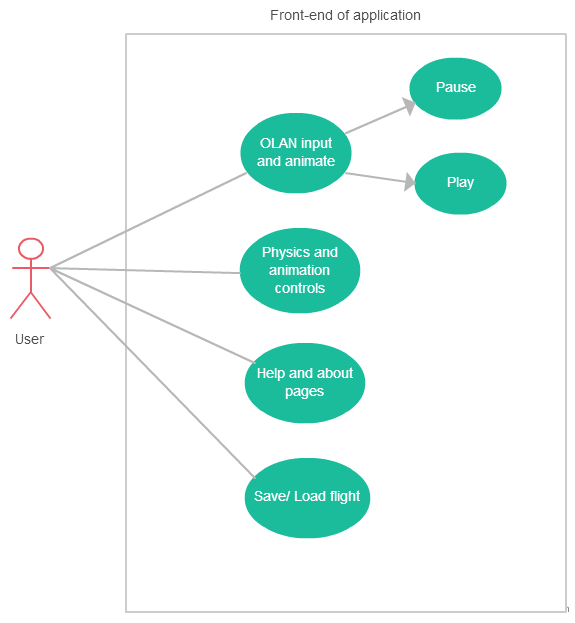
\includegraphics[width=0.8\textwidth]{images/usecase.png}
  \caption{Use-case diagram detailing user options, the canvas and OLAN input.}
  \label{fig:usecase}
\end{figure}

As you can see, there is the possibility of four sets of options each of which could have its own category in my GUI. By grouping them this way, it means the user could find the options much easier, and give a less unorganised feel to the application. Starting with the OLAN options, there are going to be two primary functions that should be required here: entering the space separated OLAN and parameters, and a drop down to allow for input from a list. The latter of which should be in its own section in the menu, whilst the first will be a simple input box at the top of the web page about the canvas. Following this, there will be the animation controls next to the input box, to begin and pause playing the flight. I have chosen the input and play button to be at the top of the page not in a menu because these will be the primary elements of the application and should be quick to use.

As for other menu pieces, there is the possibility that physics and animation related options will be available, and should be listed together in a menu. These options contain some of the extra features mentioned in my analysis, such as wind and other items that will be implemented after key functionality. Therefore, although there will be a menu for these, there may not be very many options depending on what work is complete at the end of the project. The next menu that would be required, and the last one, is the saving and loading of projects. There should be four or five options here, for saving in both formats, and loading in both formats. One of which will contain a file browser for selecting JSON files that were exported from the OLAN flight input, and then a button to begin uploading and inserting into the application. An idea alongside this would be to have some form of status bar when the application loads up a flight, depending on the size of the file. If the save files only store OLAN input and not rendered vectors, the need for the loading information would not be required.

An additional set of options, but rather extra pages will be the about and help sections. Instead of placing these alongside the other menus, these can simply sit onto the top menu bar next to the OLAN input box. Rather than options, these should be simple HTML pages that give the user some insight into the application.

It was mentioned earlier in the report about using the lazy initialisation pattern, and simply disabling options could help towards this. For example, a user may try to enter OLAN and press the play button before the manoeuvres have loaded up causing an error. An idea could be to make the input box disabled by default, and then enable it form the back-end once the application is fully loaded. To help understand this, a flow chart in figure ~\ref{fig:flow} shows what the user should be able to at what stage in loading of the application. 

\clearpage

\begin{figure}[h!]
  \centering
      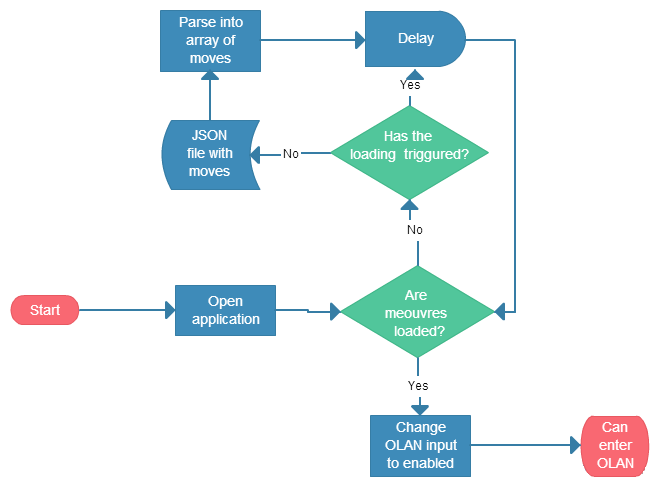
\includegraphics[width=1\textwidth]{images/flow.png}
  \caption{Flow chart showing how the application should run in accordance to loading up and then allowing the user to begin using various functions.}
  \label{fig:flow}
\end{figure}

As you can see from the flowchart above, the input box that allows OLAN entry will be disabled until loading of the aircraft model, manoeuvre JSON file and setting up of the various controllers. Options should already be enabled when loading up, as back-end checking can be performed separately to lighten the front-end. In any case, because listeners are set up last, any options in the GUI will not function until the rest of the application loads up anyway.

\subsection{CSS and wire-frame design}
Following finding of all the required use cases on the application, it is now possible to create draft wire-frame designs for the front-end of the application. Because it would be ideal that the web page works on both mobile and desktop, a CSS library could help to create this easily and quickly. After considering the two main CSS libraries used on the web (Zurb Foundation \cite{foundation} and Twitter Bootstrap \cite{bootstrap}), it was decided that the first would be more appropriate for the application due to some built in functionality that could be useful to the application. The functionality that was found to be most useful was an off-canvas menu. This menu allowed content to be hidden to the side of the page, and then when opened pushed content on the page to the right. This is especially useful for this application where getting maximum space is best for the canvas. In addition to this, the menu allowed for stacking, so it is possible to add sub menus that also push in from the left. 

Alongside the menu feature, the general appearance and flexibility of the library will give the application a more attractive and professional appearance, for example replacing check-boxes for options with sliding switches. To give a more detailed insight into the idea of what the application could look like using this library see the following wire-frame in figure ~\ref{fig:wiredesktop}.

\begin{figure}[h!]
  \centering
      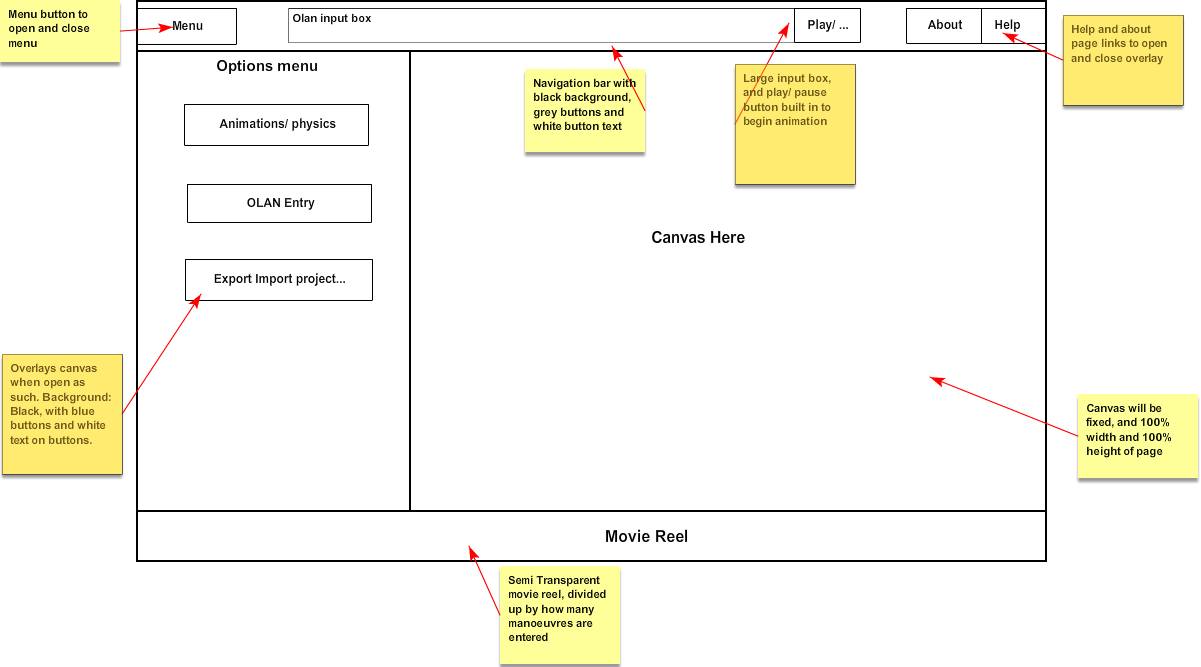
\includegraphics[width=1\textwidth]{images/desktop.png}
  \caption{Wire-frame design detailing desktop view of the application, including the open menu for the 'off canvas feature'.}
  \label{fig:wiredesktop}
\end{figure}

As well as the desktop design of the site, a design of the proposed mobile view can be found in the following figure ~\ref{fig:wiremobile}.

\begin{figure}[h!]
  \centering
      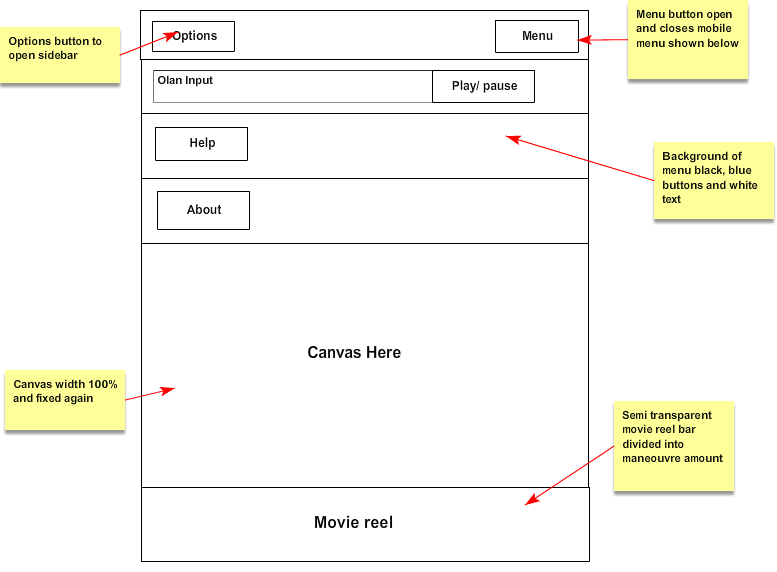
\includegraphics[height=8.5cm]{images/mobile.png}
  \caption{Wire-frame design detailing mobile view of application with navigation bar in minified version.}
  \label{fig:wiremobile}
\end{figure}

It can be seen that the mobile view follows the same style as the desktop version in the fact that menus and other elements are kept hidden away while showing the canvas for maximum space usage. Again, the off-canvas menu will be used to hide all the option menus, whilst the navigation containing the OLAN input and play button will be hidden at the top of the screen like a standard mobile navigation bar. Items like the about and help pages will take up the entire page on mobile to make text easier to scroll through, whilst on the mobile the help pages will only take around 50\% and overlay the canvas. 

In addition to both wire-frames and their respective descriptions, it should be pointed out the reasoning for colour scheme choice and other accessibility issues. It was decided that the black background with white text was best for readability and a cleaner look. If the colours were flipped, the application edges such as the navigation would not stand out enough, and finding the edge of the canvas harder. Because the foundation library is being used, it is possible to change the colour scheme from its default blue to white easily through its custom download page. It will also be endeavoured to create the site as responsive as possible, with menus and navigation elements correctly scaled on different sizes systems. This should mean the application should appear as well as a tablet than a mobile.

\section{Planned use of services}
Throughout the development of the application, it is planned that a range of tools will be explored and used to help make implementation, testing and documentation more efficient. The first of these is Github \cite{github}, which will give two features: allow version control of the development work, so to keep it safe and secure, and to provide a free web hosting service. This can be achieved by creating a 'gh-pages' branch in a repository as seen on the Github site \cite{pages}, and then any files in that branch can be navigated to on-line. This will be especially useful for my application, as after each commit, the results of changes will be reflected on this branch's web-link. Github will allow work to be carried out on any machine, and to revert any changes that may produce errors when implementing features.

Working alongside Github, a service called Travis \cite{travis} will be used to test the application. The Travis continuous development server will allow the application test files to run on each commit to the Github repository. It works by firstly linking to Github, then by reading a file in the repository containing instructions of running any test files that exist. Travis brings with it lots of useful features, as it is possible to run a wide set of different languages and libraries from the Travis file in the repository. The testing library toolkit that will be used in the development of the application will be JUnit, alongside a framework called Jasmine \cite{jasmine}. JUnit acts a lot like any other unit based test, allowing a set of tests to be run after another testing different scenarios across an applications functions. Jasmine will allow for cleaner behaviour driven testing of JavaScript code and will run headless, meaning the application can be tested without loading up the web-page.

A library that will be used during the implementation stage will be the JSDoc library \cite{jsdoc}, which will help when creating organised documentation for all the JavaScript methods and variables. It is important that each JavaScript module implemented has easily understandable comments to help future development for times when it may have become unclear what one part of the code is doing. In order to keep up with documentation, with each function that is implemented, relevant JSDoc animated comments will be added at the same stage. This means of documenting will make it effortless to create the documentation when the application is complete, by simply running the library from the command line to generate the documenting HTML pages.

Another technology that will be used to implement the application looks towards the front-end. Rather than standalone CSS for styling the web-page, Sass \cite{sass} will be used. In order to use Sass to style a page, it must be complied into its primitive CSS form before adding it to a site. Therefore, while developing the site locally, a software known as Koala \cite{koala} will be used to automatically compile the Sass file holding style information after each change to any Sass files. The main reason for using Sass follows the rule of keeping the application as maintainable as possible, and easy to understand for future referencing. As Sass uses a good layered structure, it enforces this easy readability.

The final supporting service that would be useful to have to increase productivity during development is a local server application. As I have had past experience using a program called EasyPHP \cite{easyphp}, this will be used when performing coding. The main advantage of using this is that it will be possible to edit and see the site live, rather than having to commit each time. The local server is needed due to issues loading JSON files dynamically through JavaScript which is not possible to do through simply opening the HTML file in a browser.
